\documentclass[12pt,a4paper]{article}
\usepackage[british]{babel}
\usepackage[margin=27mm]{geometry}
\usepackage{amsmath,amssymb,amsthm,mathtools,bm}
\usepackage{booktabs,graphicx,caption,subcaption}
\usepackage[authoryear,round,longnamesfirst]{natbib}
\usepackage{enumitem,microtype,setspace,flafter,placeins}
\usepackage[colorlinks=true,linkcolor=blue,citecolor=blue,urlcolor=blue]{hyperref}
\setlength{\parskip}{0.3em}
\setlength{\emergencystretch}{3em}
\setlength{\parindent}{1.25em}
\doublespacing
\captionsetup{font={stretch=1.667}}
\renewenvironment{abstract}{\begin{center}\bfseries\abstractname\end{center}\begin{quote}\normalsize}{\end{quote}}
\setlist[enumerate]{itemsep=0.2em,topsep=0.4em}
\newtheorem{theorem}{Theorem}[section]
\newtheorem{proposition}[theorem]{Proposition}
\newtheorem{lemma}[theorem]{Lemma}
\newtheorem{corollary}[theorem]{Corollary}
\theoremstyle{remark}
\newtheorem{remark}[theorem]{Remark}
\DeclareMathOperator{\tr}{tr}
\DeclareMathOperator{\diag}{diag}
\DeclareMathOperator{\rank}{rank}
\DeclareMathOperator{\dist}{dist}
\DeclareMathOperator{\argmin}{arg\,min}
\DeclareMathOperator{\argmax}{arg\,max}
\DeclareMathOperator{\conv}{conv}
\DeclareMathOperator{\KL}{KL}
\newcommand{\R}{\mathbb R}
\newcommand{\E}{\mathrm E}
\newcommand{\Pp}{\mathrm P}
\newcommand{\Id}{I_p}
\newcommand{\F}{\mathcal F}
\newcommand{\Ccal}{\mathcal C}
\newcommand{\Kcal}{\mathcal K}
\newcommand{\Acal}{\mathcal A}
\newcommand{\norm}[1]{\left\lVert#1\right\rVert}
\newcommand{\ip}[2]{\left\langle#1,#2\right\rangle}
\newcommand{\dd}{\,\mathrm d}
\newcommand{\doi}[1]{\href{https://doi.org/#1}{\nolinkurl{doi:#1}}}
\title{Likelihood estimation of Gaussian mixtures\\with one mode per component}
\author{Hien Duy Nguyen}
\date{First draft: 17 November 2026}

% Generated native R output macros.
\newcommand{\RFixedWeights}{(0.3988685,0.3450620,0.2560695)}
\newcommand{\RFixedCovariance}{\begin{pmatrix}0.9285900&-0.0575978\\-0.0575978&0.9254839\end{pmatrix}}
\newcommand{\RJointCovariance}{\begin{pmatrix}0.7563411&0.0003447\\0.0003447&0.9661067\end{pmatrix}}
\newcommand{\RFixedMatrixSlack}{3.04\times 10^{-8}}
\newcommand{\RJointViolation}{2.86\times 10^{-15}}
\newcommand{\RCVXRVersion}{1.8.1}
\newcommand{\RClarabelVersion}{0.11.2}
\newcommand{\RVersion}{4.4.0}


\begin{document}
\maketitle

\begin{abstract}
Gaussian mixture components need not correspond to modes of the mixture density. We consider finite Gaussian mixtures with an unknown common covariance and give sufficient conditions for exactly one nondegenerate mode per component. Finite matrix inequalities bound the posterior covariance of the component means, while separate radii and local trace budgets locate every possible mode. The conditions admit configurations excluded by scalar trace bounds or a common radius. We fit the certified family by likelihood using convex inner majorisation--minimisation steps. Under a constraint qualification, the iterates approach the stationary set for the density parameters and auxiliary variables certifying the conditions. For a fixed compact family, global empirical minimisers converge towards the population minimiser set; near-minimisers with a suitable vanishing tolerance recover the whole set when population optima tie. Geometric examples and small fitting checks illustrate the construction.
\end{abstract}

\noindent\textbf{Keywords:} Gaussian mixture; modal clustering; constrained likelihood;\\
majorisation--minimisation; semidefinite constraint; set consistency.

\section{Introduction}\label{sec:introduction}

Finite Gaussian mixtures are often used to describe groups of observations through their component distributions. They can also be used to estimate a density whose modes define groups through their attraction regions. These two interpretations need not give the same groups. Several Gaussian components may contribute to one mode, and a multivariate Gaussian mixture may have more modes than components. The distinction between component-based and modal clustering is developed by \citet{hennig2010} and \citet{chacon2019}, while the geometry of Gaussian mixture modes is studied by \citet{carreira2003} and \citet{ray2005}.

We consider the case in which each Gaussian component is intended to represent a distinct density peak. The desired property concerns the full mixture: there should be exactly one mode associated with each component and no additional modes elsewhere. An ordinary mixture fit does not impose this property. It is also insufficient to show that a mode exists near each component mean. Additional modes can occur between the means, so a local argument must be accompanied by a global exclusion argument.

This problem is relevant to classification when the number of components is given a substantive interpretation. A component then has two roles. It describes a local distribution of observations and identifies a particular peak of the fitted density. Requiring these roles to agree reduces the flexibility of the mixture, but makes its component count easier to interpret. The requirement is less appropriate when several Gaussians are deliberately used to approximate one non-Gaussian group. In that setting, component merging or modal clustering after density estimation may be preferable \citep{hennig2010,chacon2019,scrucca2021}.

Modality constraints have been studied in several forms. \citet{bartolucci2005} imposes unimodality constraints in normal mixture density estimation. \citet{dasgupta2021} constructs densities with a prescribed number of modes and fits them by likelihood. More recently, \citet{tancini2025} combines Gaussian components into unimodal groups using a penalised fitting procedure. These approaches establish that modality can be part of the estimation problem. Our target is more specific: each individual Gaussian is associated with a mode of the full fitted mixture. Separation-constrained Gaussian likelihood is also an established idea. \citet{jiang2023} develops an expectation--conditional maximisation procedure for univariate mixtures with constraints on adjacent mean differences. A separation constraint alone, however, does not provide the multivariate mode correspondence considered here.

Our construction uses mixtures with an unknown covariance matrix shared by all components. After whitening, the gradient of the log density is the difference between a posterior mean of the component locations and the evaluation point. Its Hessian is the corresponding posterior covariance minus the identity matrix. These identities connect mixture modes with fixed points of a posterior-mean map \citep{carreira2000,ray2005}. We bound this covariance in separate balls around the component means. A matrix bound controls curvature in each direction and can be appreciably less restrictive than a trace bound. We then use a separate argument to place every possible mode inside one of the balls.

The sufficient conditions form a certificate with three parts. First, finite semidefinite inequalities give a uniform operator bound for the posterior covariance in each ball. The number of matrix variables grows polynomially with the number of components. Second, each component has its own localisation radius, so a close pair need not determine the radius of every other component. Third, local trace budgets account for the directions in which neighbouring means contribute appreciably. These budgets also enter the global coverage argument. The resulting conditions imply that the balls are disjoint, that the posterior-mean map leaves each ball invariant, and that it is a contraction there. Hence there is exactly one nondegenerate mode in each ball.

The common covariance assumption also clarifies the role of dimension. All stationary points lie in the affine span of the whitened means, whose dimension is at most the smaller of the ambient dimension and one less than the number of components \citep{ray2005}. Thus an increase in ambient dimension, with the number of components fixed, does not create an unrestricted number of active modal directions. High dimension still matters for estimating the common covariance, estimating the mean span, and solving the constrained fitting problems. The modal calculation and the statistical cost of fitting a high-dimensional model should therefore be distinguished.

We estimate within the certified family by maximising the ordinary mixture likelihood. A whitening parameterisation makes the Gaussian complete-data log likelihood jointly concave in the transformed means and covariance coordinates \citep{barratt2023}. Convex inner bounds for the certificate then give feasible majorisation--minimisation (MM) steps. The construction follows the established EM and inner-approximation principles of \citet{dempster1977}, \citet{wu1983}, and \citet{scutari2016}. Its role here is to make the proposed modal conditions compatible with likelihood fitting.

The fitting and statistical conclusions concern different solution sets. For a fixed sample, we prove convergence towards the Karush--Kuhn--Tucker (KKT) set of the constrained programme including its certificate variables, under an explicit constraint qualification. For increasing sample size, we study global minimisers of the negative average log likelihood over the same fixed compact family. Exact empirical minimisers approach the population minimiser set. If several distinct population densities attain the same optimum, a suitable vanishing tolerance is needed to recover the whole set in Hausdorff distance. These results adapt standard extremum-estimation and variational principles to the certified family \citep{newey1994,rockafellar1998}. They also make clear which statistical claims require a global likelihood gap in addition to an MM stopping rule.

\section{The mixture model and its modal geometry}\label{sec:geometry}

Let $[K]=\{1,\ldots,K\}$, where $K\ge2$, and let $p\ge1$. We consider densities
\begin{equation}\label{eq:mixture}
 f_\theta(x)=\sum_{j=1}^K\pi_j\phi_p(x;\mu_j,C),
 \qquad x\in\R^p,
\end{equation}
where $\pi_j>0$, $\sum_j\pi_j=1$, $\mu_j\in\R^p$, and $C$ is positive definite. Here $\phi_p(\,\cdot\,;\mu,C)$ denotes the Gaussian density with mean $\mu$ and covariance $C$, and $\theta=(\pi,\mu,C)$ collects the density parameters. A mode means a local maximum of the density. Our conclusion will exclude degenerate local maxima as well as additional strict modes.

Choose a triangular matrix $B$ with positive diagonal such that $BCB^\top=I_p$, and put $y=Bx$ and $v_j=B\mu_j$. Then
\[
 f_\theta(x)=|\det B|g(Bx),\qquad
 g(y)=\sum_{j=1}^K\pi_j\phi_p(y;v_j,I_p).
\]
The invertible transformation preserves the number and type of stationary points. Define the posterior weights, their mean, and their covariance by
\begin{align}
 w_j(y)&=\frac{\pi_j\phi_p(y;v_j,I_p)}{g(y)},&
 T(y)&=\sum_jw_j(y)v_j,\label{eq:posterior}\\
 V(y)&=\sum_jw_j(y)\{v_j-T(y)\}\{v_j-T(y)\}^{\top}.\nonumber
\end{align}
Direct differentiation gives
\begin{equation}\label{eq:derivatives}
 \nabla\log g(y)=T(y)-y,\qquad
 DT(y)=V(y),\qquad
 \nabla^2\log g(y)=V(y)-I_p.
\end{equation}
Consequently, a stationary point is a fixed point of $T$. At a local maximum, including a degenerate one, $V(y)\preceq I_p$. The notation $A\preceq D$ means that $D-A$ is positive semidefinite.

Write
\[
 q=\min(p,K-1),\qquad
 \delta_{jh}=v_h-v_j,\qquad d_{jh}=\|\delta_{jh}\|,
 \qquad D_j=\min_{h\ne j}d_{jh}.
\]
All stationary points lie in the convex hull of the $v_j$. Moreover, $\rank V(y)\le q$, so at a local maximum
\begin{equation}\label{eq:coarse}
 \tr V(y)\le q,\qquad
 \min_j\|y-v_j\|^2\le\sum_jw_j(y)\|y-v_j\|^2
 =\tr V(y)\le q.
\end{equation}
This gives a preliminary localisation bound that requires no separation condition.

To control the weights inside a ball about $v_j$, define
\begin{equation}\label{eq:odds}
 A_{jh}(s)=\frac{\pi_h}{\pi_j}
       \exp\{-d_{jh}^2/2+s d_{jh}\},\qquad s\ge0.
\end{equation}
If $\|y-v_j\|\le s$, then $w_h(y)\le A_{jh}(s)w_j(y)$. We therefore introduce the posterior-weight polytope
\begin{equation}\label{eq:polytope}
 \mathcal P_j(s)=\left\{w\in[0,1]^K:
       \sum_hw_h=1,\quad w_h\le A_{jh}(s)w_j\ (h\ne j)\right\}.
\end{equation}
For any $w$ in this polytope, put
\begin{equation}\label{eq:displacement}
 m_j(w)=\sum_{h\ne j}w_h\delta_{jh},\qquad
 \Sigma_j(w)=\sum_{h\ne j}w_h\delta_{jh}\delta_{jh}^{\top}
                  -m_j(w)m_j(w)^\top.
\end{equation}
At the actual posterior weights, these are $T(y)-v_j$ and $V(y)$, respectively. The polytope is an outer approximation to the weights attained within the ball. A bound valid throughout this larger set will also be useful for proving that $T$ maps the ball into itself.

\section{A finite certificate for one mode per component}\label{sec:certificate}

Fix $0<\beta<1$ and $\tau>0$. The constant $\beta$ bounds the local curvature through $V$, while $\tau$ supplies a strict separation margin. We allow each component to have a radius $r_j\in(0,1]$ and a trace budget $\nu_j\ge1$. These are auxiliary quantities used to certify the fitted density.

Related fixed-point arguments occur in continuous Hopfield networks. \citet[Appendix A.1.5.3]{ramsauer2021} gives invariant neighbourhoods and local contraction near sufficiently separated stored patterns; its Appendix A.1.9 makes the Gaussian-mixture connection explicit. \citet[Lemma 3.4 of the author version]{beise2026} establishes instability of fixed points away from all patterns under geometric conditions on unit-length patterns and sufficiently large scaling. These results provide precedents for local attraction and global exclusion. The conditions developed here give explicit finite bounds that can be imposed during mixture likelihood fitting.

\subsection{Directional control of the posterior covariance}

A trace bound controls $\lambda_{\max}(V)$ because $V$ is positive semidefinite, but it adds curvature across all directions. The following matrix inequalities avoid this addition.

\begin{proposition}[Finite matrix bound]\label{prop:matrix}
For a fixed component $j$ and radius $r_j$, suppose there are a vector $c_j\in\R^p$ and matrices $\Lambda_{jh}\succeq0$, $h\ne j$, such that
\begin{align}
 c_jc_j^\top+\sum_{h\ne j}A_{jh}(r_j)\Lambda_{jh}
      &\preceq\beta I_p,\label{eq:matrix1}\\
 (\delta_{jh}-c_j)(\delta_{jh}-c_j)^\top
      &\preceq\beta I_p+\Lambda_{jh},\qquad h\ne j.\label{eq:matrix2}
\end{align}
Then $\Sigma_j(w)\preceq\beta I_p$ for every $w\in\mathcal P_j(r_j)$.
\end{proposition}

\begin{proof}
Multiply \eqref{eq:matrix2} by $w_h$, sum over $h\ne j$, and include the term $w_jc_jc_j^\top$. Equation \eqref{eq:matrix1} then gives
\[
 w_jc_jc_j^\top+
 \sum_{h\ne j}w_h(\delta_{jh}-c_j)(\delta_{jh}-c_j)^\top
 \preceq \beta I_p+
 \sum_{h\ne j}\{w_h-A_{jh}(r_j)w_j\}\Lambda_{jh}
 \preceq\beta I_p.
\]
Subtracting $\{m_j(w)-c_j\}\{m_j(w)-c_j\}^\top$ proves the result.
\end{proof}

For a fixed density and radii, these conditions are a semidefinite feasibility problem. For example, \eqref{eq:matrix2} is equivalent to
\[
 \begin{pmatrix}
  \beta I_p+\Lambda_{jh}&\delta_{jh}-c_j\\
  (\delta_{jh}-c_j)^\top&1
 \end{pmatrix}\succeq0.
\]
The first inequality has an analogous Schur-complement representation. There are $K(K-1)$ multiplier matrices, rather than an enumeration of the $2^{K-1}$ vertices associated with independent odds bounds for each component. The conditions are sufficient; they are not asserted to characterise every covariance bound on $\mathcal P_j(r_j)$. Sufficient semidefinite treatment of matrix uncertainty has a broader history \citep{bental2002}. Proposition~\ref{prop:matrix} gives the particular construction needed here.

\subsection{Local trace budgets}

The global localisation bound \eqref{eq:coarse} uses $q$. It can be conservative when the nearby means vary mainly along a smaller number of directions and other components are remote. To account for this, choose a symmetric matrix $M_j$ with $0\preceq M_j\preceq I_p$ and require
\begin{equation}\label{eq:budget}
 \tr M_j+\frac1\beta\sum_{h\ne j}A_{jh}(\sqrt q)
            \delta_{jh}^\top(I_p-M_j)\delta_{jh}\le\nu_j.
\end{equation}
The trace of $M_j$ pays for the directions retained by this matrix. The remaining directions are weighted by coarse posterior-odds bounds. The radius $\sqrt q$ in these bounds comes from \eqref{eq:coarse}; thus the budget can be used before the sharper localisation has been proved.

For a fixed density, define
\[
 W_j=\sum_{h\ne j}A_{jh}(\sqrt q)\delta_{jh}\delta_{jh}^\top.
\]
The smallest admissible trace budget obtained by varying $0\preceq M_j\preceq I_p$ is
\begin{equation}\label{eq:spectralbudget}
 \nu_j^*=\max\left\{1,\sum_{\ell=1}^p
                \min\{1,\lambda_\ell(W_j)/\beta\}\right\}\le q.
\end{equation}
A minimising $M_j$ is the orthogonal projector onto eigendirections of $W_j$ with eigenvalues exceeding $\beta$. At equality either choice is possible. The formula provides a convenient way to check or initialise a certificate. During fitting we update $M_j$ jointly with the other variables.

The budget has two uses. At a hypothetical mode assigned to its nearest mean $v_j$, it gives $\tr V\le\nu_j$. On the local posterior polytope, when the matrix bound also holds, it gives $\tr\Sigma_j\le\beta\nu_j$. The first inequality locates all modes; the second helps establish invariance of each ball. Both are proved in Appendix~\ref{app:geometry}.

\subsection{Global coverage and invariance}

Require, for every ordered pair $j\ne h$,
\begin{equation}\label{eq:separation}
 d_{jh}^2\ge \nu_j+1+\tau+r_j^2+\frac{\nu_j}{r_j^2}.
\end{equation}
This condition couples the radius and the trace budget to the relevant pairwise separation. It implies $d_{jh}^2\ge4+\tau$, so the closed balls
$\mathbb B_j=\{y:\|y-v_j\|\le r_j\}$ are disjoint.

For $D^2>2(\nu+1)$ and $\nu\ge1$, define
\begin{equation}\label{eq:rho}
 \rho(D,\nu)^2=
 \frac{2\nu}{D^2-\nu-1+
          \sqrt{(D^2-\nu-1)^2-4\nu}}.
\end{equation}
This is the smaller root of a quadratic arising from the covariance decomposition between one component and the remaining components.

\begin{theorem}[One mode per component]\label{thm:modes}
Suppose that \eqref{eq:matrix1}, \eqref{eq:matrix2}, \eqref{eq:budget}, and \eqref{eq:separation} hold for every component, with $0<r_j\le1$, $\nu_j\ge1$, $\Lambda_{jh}\succeq0$, and $0\preceq M_j\preceq I_p$. Then $f_\theta$ has exactly $K$ modes. They are nondegenerate, and the $j$th mode lies in
\[
 \mathcal E_j=\{x:\|B(x-\mu_j)\|<r_j\}.
\]
In whitened coordinates, $T$ maps $\mathbb B_j$ into its interior and is a contraction there with constant at most $\beta$. Iteration of $T$ from any point of $\mathbb B_j$ converges to its unique mode. In addition, throughout $\mathbb B_j$,
\begin{equation}\label{eq:invariance}
 w_j(y)>\tfrac12,\qquad
 \|T(y)-v_j\|
 \le\sqrt\beta\,\rho(D_j/\sqrt\beta,\nu_j)
 <\rho(D_j,\nu_j)<r_j.
\end{equation}
Every local maximum lies in one of these balls.
\end{theorem}

The proof has two distinct steps. At any possible mode, the preliminary bound \eqref{eq:coarse} makes the local budget available. A covariance decomposition then forces its distance from the nearest mean below $\rho(D_j,\nu_j)$. This excludes modes outside the balls. Inside each ball, Proposition~\ref{prop:matrix} bounds $DT$. The same bound over the whole posterior polytope, together with the local trace budget, establishes \eqref{eq:invariance}. The contraction theorem then supplies one fixed point per ball. The details are given in Appendix~\ref{app:geometry}.

The association in Theorem~\ref{thm:modes} is stronger than an equality of counts: a specified component has a specified nearby mode, and starting mean shift at its mean locates that mode. A component mean generally differs from the mode of the full density. The theorem also does not identify the maximum-posterior component partition with the attraction-basin partition used in modal clustering.

\subsection{Relation to scalar bounds and dimension}

The matrix construction contains a useful scalar trace construction. Suppress $j$, write $A_h=A_{jh}(r_j)$, $S=\sum_{h\ne j}A_h$, and suppose $S<1$. Let the saturated weights be $w_j^*=1/(1+S)$ and $w_h^*=A_h/(1+S)$ for $h\ne j$. Put
\[
 c=m_j(w^*),\qquad
 \Gamma=\tr\Sigma_j(w^*).
\]
If $\Gamma\le\beta$ and $d_{jh}>2\sqrt\beta$ for every $h\ne j$, then
\begin{equation}\label{eq:scalarwitness}
 \Lambda_{jh}=\{\|\delta_{jh}-c\|^2-\beta\}I_p
\end{equation}
gives feasible matrix witnesses. The proof is in Appendix~\ref{app:geometry}. A configuration with a feasible matrix certificate but $\Gamma>1$ will be given in Section~\ref{sec:examples}. The directional construction therefore admits densities excluded by this scalar condition.

For a fixed density, the certificate can be checked in the affine span of the whitened means. If its dimension is $s$, choose an orthonormal basis $U$ for the mean differences and write $v_j=b+Ua_j$, with $b$ orthogonal to that span. Completing $U$ by $U_\perp$ gives
\begin{equation}\label{eq:factorisation}
 g(y)=
 \phi_{p-s}\{U_\perp^\top(y-b);0,I_{p-s}\}
 \sum_j\pi_j\phi_s\{U^\top(y-b);a_j,I_s\}.
\end{equation}
The complementary factor is omitted if $s=p$. Compressing $c_j$, $\Lambda_{jh}$ and $M_j$ to this span preserves feasibility or reduces the trace budget; embedding reduced witnesses with zero complementary blocks gives the converse. The coarse caps remain $A_{jh}(\sqrt q)$. This establishes an exact reduction for checking a fixed density. Joint fitting uses the ambient coordinates because the span itself varies with the means.

\section{Likelihood estimation within the certified family}\label{sec:fitting}

\subsection{A common parameter space for computation and inference}

Use logits $\alpha_j$ with $\alpha_K=0$ and
$\pi_j=\exp(\alpha_j)/\sum_h\exp(\alpha_h)$. Let
$\eta=(B,v,\alpha)$ be the density coordinates. Choose a fixed deterministic convex compact envelope for $\eta$, with a positive lower bound on each diagonal element of the triangular $B$. This bounds the original means and the covariance eigenvalues and bounds the weights away from zero.

For fitting, introduce scalar caps $a_{jh}\ge A_{jh}(r_j)$ and replace the corresponding odds in \eqref{eq:matrix1} by $a_{jh}$. This leaves the represented density family unchanged: setting $a_{jh}=A_{jh}(r_j)$ is allowed, and decreasing a feasible cap to this value only reduces the positive semidefinite sum. Define the complete optimisation variable
\[
 z=(\eta,r,\nu,c,a,\Lambda,M).
\]
The variables after $\eta$ are witnesses that certify the density; they are not additional mixture components.

Let $\mathcal C$ be a convex compact base containing the density envelope and the restrictions $r_j\le1$, $\nu_j\ge1$, $\Lambda_{jh}\succeq0$, and $0\preceq M_j\preceq I_p$. The witness bounds needed for compactness can be chosen redundant. Indeed, if $D_{\max}$ bounds all pair distances and $D_0=\sqrt{4+\tau}$, the exact constraints imply
\begin{equation}\label{eq:witnessbounds}
 r_j\ge D_{\max}^{-1},\qquad
 \nu_j\le\frac{D_{\max}^2-2-\tau}{2},\qquad
 \|c_j\|\le\sqrt\beta.
\end{equation}
They also bound $a$ and $\Lambda$, as shown in Appendix~\ref{app:compactness}. Wider closed bounds may therefore be included in $\mathcal C$ without excluding a feasible point.

Let $\mathcal F$ be the subset of $\mathcal C$ satisfying
\begin{equation}\label{eq:exactlift}
\begin{aligned}
 A_{jh}(r_j)&\le a_{jh},\\
 c_jc_j^\top+\sum_{h\ne j}a_{jh}\Lambda_{jh}&\preceq\beta I_p,\\
 (\delta_{jh}-c_j)(\delta_{jh}-c_j)^\top&\preceq\beta I_p+\Lambda_{jh},\\
 \tr M_j+\beta^{-1}\sum_{h\ne j}A_{jh}(\sqrt q)
       \delta_{jh}^\top(I_p-M_j)\delta_{jh}&\le\nu_j,\\
 \nu_j+1+\tau+r_j^2+\nu_j/r_j^2&\le d_{jh}^2.
\end{aligned}
\end{equation}
All pairwise conditions apply to ordered pairs. Assume $\mathcal F$ is nonempty, and set
\[
 \Theta=\{\theta(z):z\in\mathcal F\},\qquad
 \theta(z)=\left(\pi(\alpha),B^{-1}v,B^{-1}B^{-\top}\right).
\]
Both $\mathcal F$ and $\Theta$ are compact. We use this same $\Theta$ for the estimator and its population target.

For observations $X_1,\ldots,X_n$, define
\begin{equation}\label{eq:empiricalrisk}
 R_n(\theta)=-\frac1n\sum_{i=1}^n\log f_\theta(X_i).
\end{equation}
The constrained maximum likelihood estimators minimise $R_n$ over $\Theta$. Equivalently, one can minimise $R_n(z)=R_n\{\theta(z)\}$ over $\mathcal F$. The global optimum exists by compactness. The criterion is the ordinary mixture likelihood; the modal restrictions enter through the feasible family.

\subsection{A convex inner MM step}

At a current feasible point $z_t$, let $R_{ij}^t$ be the posterior responsibility of component $j$ for $X_i$, and put $N_j^t=\sum_iR_{ij}^t$. Up to constants independent of a trial point $u$, the EM auxiliary function is
\begin{equation}\label{eq:Q}
\begin{aligned}
 Q_n(u\mid z_t)
 ={}&n\sum_{b=1}^p\log B_{u,bb}
 -\frac12\sum_{i,j}R_{ij}^t\|B_uX_i-v_{u,j}\|^2\\
 &+\sum_jN_j^t\alpha_{u,j}
       -n\log\sum_h\exp(\alpha_{u,h}).
\end{aligned}
\end{equation}
Each term is concave in the trial density coordinates. For $\gamma>0$, define
\begin{equation}\label{eq:H}
 H_n(u\mid z_t)=R_n(z_t)
 -\frac{Q_n(u\mid z_t)-Q_n(z_t\mid z_t)}n
 +\frac\gamma2\|u-z_t\|^2.
\end{equation}
The norm uses Euclidean norms for vector coordinates and Frobenius norms for symmetric matrices. It includes all certificate variables but excludes temporary solver epigraph variables. The function $H_n$ is strongly convex, touches $R_n$ at $z_t$, has the same first derivative there, and satisfies
\begin{equation}\label{eq:EMbound}
 R_n(u)\le H_n(u\mid z_t)-\frac\gamma2\|u-z_t\|^2.
\end{equation}

The constraints in \eqref{eq:exactlift} are nonconvex jointly. We replace them by convex upper bounds that agree in value and derivative at $z_t$. Four constructions suffice.

\paragraph{Posterior-odds caps.}
For one pair, let $\delta_t$ and $r_t$ be the current displacement and radius, $d_t=\|\delta_t\|$, $e_t=\delta_t/d_t$, and $b_t=d_t-r_t$. Then
\[
 L_t(\delta,r)=b_t(e_t^\top\delta-r)-b_t^2/2-r^2/2
 \le \|\delta\|^2/2-r\|\delta\|.
\]
Hence the convex constraint
\begin{equation}\label{eq:innerodds}
 a_{jh}\ge\exp\{\alpha_h-\alpha_j-L_t(\delta_{jh},r_j)\}
\end{equation}
implies the exact cap constraint.

\paragraph{Matrix products.}
For a fixed $\kappa>0$, put
\begin{equation}\label{eq:matrixmajorant}
\begin{aligned}
 \mathcal U_t(a,\Lambda)
 ={}&a_t\Lambda+a\Lambda_t-a_t\Lambda_t\\
 &+\frac14\left\{\sqrt\kappa(a-a_t)I_p+
                 \frac{\Lambda-\Lambda_t}{\sqrt\kappa}\right\}^2.
\end{aligned}
\end{equation}
The difference $\mathcal U_t(a,\Lambda)-a\Lambda$ is the positive semidefinite square obtained by changing the plus sign inside braces to a minus sign. Replacing $a\Lambda$ by $\mathcal U_t$ in the first matrix constraint gives a convex matrix inequality. Its squared terms have Schur-complement epigraphs. The second matrix constraint in \eqref{eq:exactlift} is already convex and is retained.

\paragraph{Local trace budgets.}
Fix $0<\varrho<D_0/2$ and restrict $\|\delta_{jh}-\delta_{jh}^t\|\le\varrho$. Write $\xi=(\delta,s,M)$, where $s=\alpha_h-\alpha_j$, and let
\begin{equation}\label{eq:h}
 h(\xi)=\exp\{s-\|\delta\|^2/2+\sqrt q\|\delta\|\}
               \delta^\top(I_p-M)\delta.
\end{equation}
Choose a positive upper bound $L_h$ for the Hessian norm of $h$ on every permitted segment from anchor to trial. Such a bound is finite because the distances stay away from zero and the parameter envelope is compact. An explicit bound is given in Appendix~\ref{app:algorithm}. The quadratic function
\begin{equation}\label{eq:hhat}
 \widehat h(\xi\mid\xi_t)
 =h(\xi_t)+Dh(\xi_t)[\xi-\xi_t]
             +\frac{L_h}{2}\|\xi-\xi_t\|^2
\end{equation}
majorises $h$. We impose
\[
 \tr M_j+\beta^{-1}\sum_{h\ne j}
       \widehat h(\xi_{jh}\mid\xi_{jh}^t)\le\nu_j.
\]
This updates $M_j$ jointly with the other variables, including when a residual quadratic form is zero. The support is continuous in the anchor, which is needed for the convergence result.

\paragraph{Separation and radii.}
Young's inequality gives a convex tangent upper bound for $\nu/r^2$. Combining it with an affine lower bound for $\|\delta\|^2$ yields
\begin{equation}\label{eq:innersep}
 1+\tau+\nu_j+r_j^2+
 \frac{\nu_j^2}{2\nu_j^t(r_j^t)^2}
 +\frac{\nu_j^t(r_j^t)^2}{2r_j^4}
 \le2(\delta_{jh}^t)^\top\delta_{jh}-(d_{jh}^t)^2.
\end{equation}

Let $\mathcal K(z_t)$ be the convex set formed by these inner constraints and the base $\mathcal C$. Each support is tight at the anchor, so
\[
 z_t\in\mathcal K(z_t)\subseteq\mathcal F.
\]
The next trial point and accepted point are
\begin{equation}\label{eq:update}
 u_t=\argmin_{u\in\mathcal K(z_t)}H_n(u\mid z_t),\qquad
 z_{t+1}=z_t+\lambda_t(u_t-z_t),
 \quad 0<\lambda_{\min}\le\lambda_t\le1.
\end{equation}
Strong convexity makes $u_t$ unique. Full steps and a fixed retreat fraction are both allowed. Every iterate remains certified and the likelihood is nondecreasing.

\subsection{Convergence of the fitting iteration}

The regularity condition below concerns the boundary of the optimisation problem. It is separate from the margins that control the spatial modes.

Write the smooth non-base constraints in \eqref{eq:exactlift} as $g_i(z)\le0$ and $G_k(z)\preceq0$. At each cluster point $z$, assume that there is a direction $d$ such that $z+sd\in\mathcal C$ for all sufficiently small $s>0$,
\begin{equation}\label{eq:CQ}
 Dg_i(z)[d]<0\quad\text{for every active scalar constraint},\qquad
 E_k^\top DG_k(z)[d]E_k\prec0
\end{equation}
for every matrix constraint with a nonzero nullspace spanned by $E_k$. Fixed equalities are handled in the affine hull of $\mathcal C$, and identically satisfied non-base constraints are removed. This is a relative strict linearised feasibility condition.

Let $\mathcal S_n^{\mathrm{lift}}$ be the KKT set for minimising $R_n(z)$ over $\mathcal F$, with normal cones to $\mathcal C$ and positive semidefinite multipliers for the matrix constraints.

\begin{theorem}[Convergence to the lifted stationary set]\label{thm:MM}
For a fixed sample, start \eqref{eq:update} at $z_0\in\mathcal F$. Use fixed positive $\gamma$, $\kappa$, and valid curvature bounds, with the stated trust radius and step fractions. If \eqref{eq:CQ} holds at every cluster point, then $R_n(z_t)$ decreases to a finite value and
\[
 \dist(z_t,\mathcal S_n^{\mathrm{lift}})\longrightarrow0.
\]
Every cluster point is a lifted KKT point. The cluster set is compact and connected, and $R_n$ is constant on it. If the stationary points at the attained objective value are isolated, $z_t$ converges to one point. Every iterate and parameter limit represents a density with exactly $K$ nondegenerate modes.
\end{theorem}

The proof in Appendix~\ref{app:algorithm} uses both sufficient decrease and continuity of the changing inner feasible sets. The constraint qualification supplies the strict feasible points needed for the latter step. Monotonicity of the likelihood alone would not establish the theorem.

Inexact convex solves give the same conclusion if the trial point is inner feasible,
\[
 H_n(u_t\mid z_t)\le R_n(z_t),\qquad
 H_n(u_t\mid z_t)-\min_{u\in\mathcal K(z_t)}H_n(u\mid z_t)
 \le\varepsilon_t,\qquad \varepsilon_t\to0.
\]
A valid primal--dual bound can certify this convex subproblem gap. A fixed nonzero tolerance does not establish the asymptotic condition.

The stationary set is that of the programme including its witnesses. A stationary point in these coordinates need not be stationary after the witnesses are eliminated: another witness for the same density can expose a feasible improving direction. It also need not be a global likelihood optimum. These distinctions are material because the likelihood remains nonconvex. The statistical results below concern global minimisers or fits with a vanishing global objective gap.

\section{Population targets and empirical solution sets}\label{sec:statistics}

\subsection{The target within a fixed certified family}

Let $X_1,X_2,\ldots$ be IID with law $P$ on $\R^p$, and keep $K$, $p$, the margins, and the compact parameter envelope fixed. Assume $\E_P\|X\|^2<\infty$. Define
\begin{equation}\label{eq:population}
 R(\theta)=\E_P\{-\log f_\theta(X)\},\qquad
 \mathcal A=\argmin_{\theta\in\Theta}R(\theta),\qquad
 \mathcal A_n=\argmin_{\theta\in\Theta}R_n(\theta).
\end{equation}
Both minimiser sets are nonempty and compact. Every density in the population target retains the mode correspondence of Theorem~\ref{thm:modes}.

If $P$ has density $p_0$ and finite Kullback--Leibler divergence to a member of the family, then $\mathcal A$ consists of its best Kullback--Leibler approximations within $\Theta$. This is the usual misspecified likelihood interpretation \citep{white1982}. Under correct specification, the target density is $p_0$. The common-covariance mixture with distinct means is identifiable up to label permutations; a direct argument for this setting is included in Appendix~\ref{app:statistics}. The sufficient certificate can exclude other mixtures that already have exactly $K$ modes, so correct specification means membership in $\Theta$ itself.

Uniformly over $\Theta$, there are finite constants $c_1,c_2$ such that
\[
 |\log f_\theta(x)|\le c_1+c_2\|x\|^2.
\]
Continuity and compactness then give the uniform strong law
\begin{equation}\label{eq:ULLN}
 U_n=\sup_{\theta\in\Theta}|R_n(\theta)-R(\theta)|
       \longrightarrow0\qquad\text{almost surely}.
\end{equation}
The Gaussian envelope and proof are provided in Appendix~\ref{app:statistics}.

\subsection{Directed and Hausdorff convergence}

For nonempty compact sets $D,E$ in the parameter space, write
\[
 e(D,E)=\sup_{\theta\in D}\dist(\theta,E),\qquad
 d_H(D,E)=\max\{e(D,E),e(E,D)\}.
\]
The directed distance $e(D,E)$ asks whether every point of $D$ is close to $E$. Hausdorff distance also asks whether all of $E$ is represented by nearby points of $D$.

For $a\ge0$, define the near-minimiser sets
\[
 \mathcal A_n(a)=\{\theta\in\Theta:
        R_n(\theta)\le\min_\Theta R_n+a\},\qquad
 \mathcal A(a)=\{\theta\in\Theta:
        R(\theta)\le\min_\Theta R+a\}.
\]
Set $\mathcal A(a)=\varnothing$ for $a<0$, and let
$\omega(a)=\sup_{\theta\in\mathcal A(a)}\dist(\theta,\mathcal A)$ for $a\ge0$.
Compactness gives $\omega(a)\to0$ as $a\downarrow0$.

\begin{theorem}[Consistency of likelihood solution sets]\label{thm:sets}
Under the conditions of this section,
\[
 \left|\min_\Theta R_n-\min_\Theta R\right|\le U_n,\qquad
 \mathcal A(a-2U_n)\subseteq\mathcal A_n(a)
                    \subseteq\mathcal A(a+2U_n).
\]
Consequently, for any nonnegative $a_n\to0$ almost surely,
\begin{equation}\label{eq:outer}
 e\{\mathcal A_n(a_n),\mathcal A\}
 \le\omega(a_n+2U_n)\longrightarrow0
 \qquad\text{almost surely}.
\end{equation}
If $a_n>0$, $a_n\to0$, and $U_n/a_n\to0$ almost surely, then
\begin{equation}\label{eq:hausdorff}
 d_H\{\mathcal A_n(a_n),\mathcal A\}\longrightarrow0
 \qquad\text{almost surely}.
\end{equation}
If the population target is unique in a chosen quotient space, the exact empirical minimiser sets converge in Hausdorff distance in that space.
\end{theorem}

The exact sets correspond to $a_n=0$ and always satisfy the directed conclusion. They need not converge in Hausdorff distance when distinct population optima tie. Small empirical perturbations can select one optimum and omit another. A near-minimiser set includes every population minimiser once $a_n\ge2U_n$ and still excludes points separated from the target as $a_n\to0$. This is why the tolerance gives the stronger conclusion.

For a unique density target, one may work directly with densities in $L_1$, or with parameters modulo label permutations. If the parameter envelope is invariant under label permutations, the equivalent labelled representatives can also be retained. No such invariance is assumed merely from using a logit parameterisation.

\begin{corollary}[An explicit tolerance]\label{cor:tolerance}
If $\E_P\|X\|^4<\infty$, then
\[
 U_n=O_P(n^{-1/2}),\qquad
 U_n=o_{\mathrm{a.s.}}\{\log(en)/\sqrt n\}.
\]
Thus $a_n=\log(en)/\sqrt n$, on the negative average log-likelihood scale, satisfies \eqref{eq:hausdorff}.
\end{corollary}

The rate follows from a Lipschitz bound for the Gaussian log likelihood on the compact envelope and a maximal-moment argument; the details are in Appendix~\ref{app:statistics}. It is a fixed-dimensional statement.

\subsection{Modes and computed fits}

At a certified mode, \eqref{eq:derivatives} gives
\begin{equation}\label{eq:curvature}
 \nabla_x^2\log f_\theta
 \preceq-(1-\beta)C^{-1}.
\end{equation}
The covariance envelope therefore keeps the mode curvature away from zero. The implicit function theorem and the disjoint localisation imply that the unordered mode set varies continuously with $\theta$. The directed and Hausdorff set conclusions consequently transfer to the corresponding collections of density and mode configurations. Under correct specification, a unique target density gives consistent estimation of its modes.

For a computed feasible fit $\widehat\theta_n$, let
\[
 g_n=R_n(\widehat\theta_n)-\min_{\theta\in\Theta}R_n(\theta)
\]
be its global objective gap. Then
\begin{equation}\label{eq:gap}
 0\le R(\widehat\theta_n)-\min_\Theta R\le g_n+2U_n.
\end{equation}
Hence $g_n\to0$ implies consistency towards $\mathcal A$, in the same mode of convergence. The MM theorem controls a convex subproblem gap and the lifted stationary set; it does not establish $g_n\to0$. Equation \eqref{eq:gap} states the additional condition needed to connect a computed sequence to the global statistical target.

\section{Numerical illustrations}\label{sec:examples}

The examples separate three sources of conservatism: summing curvature across directions, imposing one radius on all components, and using the full rank bound for every local configuration. All stated mode counts follow from the certificate. Numerical values illustrate the inequalities; the supplied R code also contains exact rational sign checks for the strict geometric examples.

\subsection{A matrix bound where the scalar trace bound fails}

Consider three equally weighted components in two dimensions with covariance $I_2$ and means at the vertices of an equilateral triangle of side length $d=2.8$. Take
\[
 \beta=0.99,\qquad \tau=0.01,\qquad
 r_j=0.68,\qquad \nu_j=2,\qquad M_j=I_2.
\]
In coordinates centred at one vertex and directed towards the midpoint of the opposite side, the other two displacements are
$\delta_\pm=(\sqrt3d/2,\pm d/2)^\top$.
Both odds caps equal $A=\exp(-2.016)=0.1331871496\ldots$.
The witnesses
\[
 c=(0.51,0)^\top,\qquad
 \Lambda_\pm=
 \begin{pmatrix}2.72&\pm2.70\\ \pm2.70&2.70\end{pmatrix}
\]
satisfy the matrix inequalities. Rotating them gives the witnesses at the other vertices. Interval checks give a first-matrix slack greater than $0.00536$, positive multiplier determinants exceeding $0.05399$, and second-matrix slack determinants exceeding $0.07448$. The squared-separation slack exceeds $0.04234$.

At the saturated posterior weights, the two covariance eigenvalues are approximately $0.97666465$ and $0.41227434$. Their sum is $1.38893899$. The smaller admissible radius under the same separation margin is $0.67630839$, at which the trace is still $1.37973593$. Thus the scalar trace condition fails for every admissible radius and every $\beta<1$, whereas the finite matrix certificate proves that the mixture has exactly three modes.

\begin{figure}[t]
 \centering
 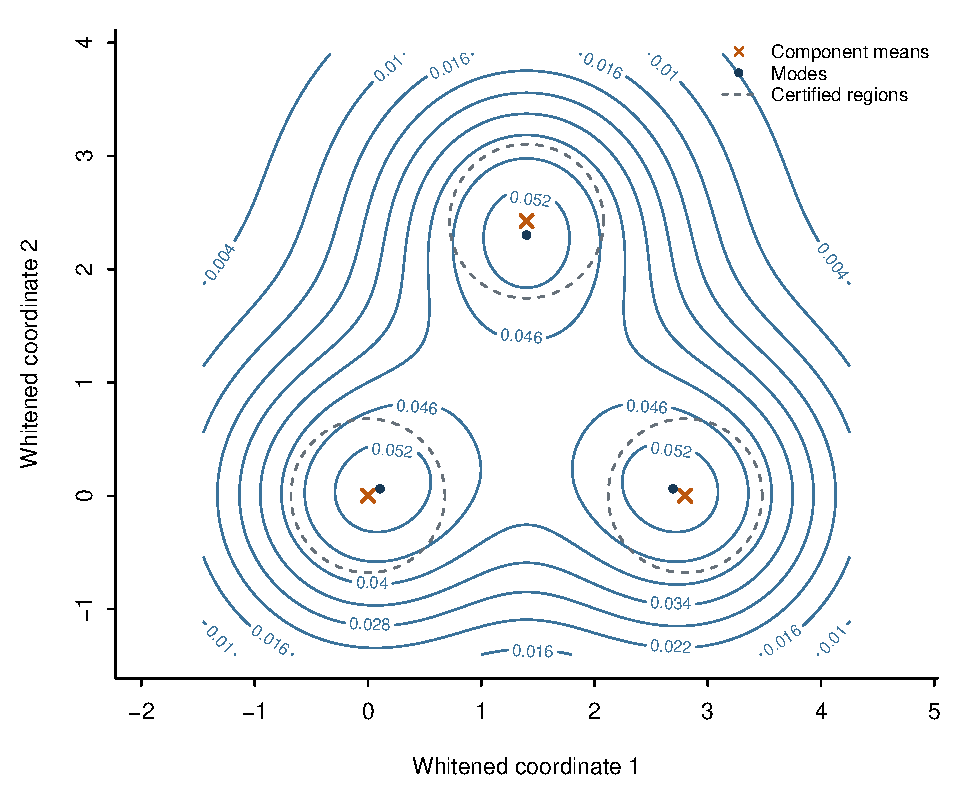
\includegraphics[width=0.86\textwidth]{figures/triangle_modes.pdf}
 \caption{The equal-weight Gaussian mixture with identity covariance and an equilateral configuration of side length $2.8$. Crosses mark component means, filled circles mark modes found by posterior-mean iteration, and dashed circles show the certified radius $0.68$. Density contours are evaluated directly from the mixture in R. The certificate, rather than the numerical root search, establishes that the three displayed modes are exhaustive.}
 \label{fig:triangle}
\end{figure}
\FloatBarrier

\subsection{Separate radii for an isolated component}

Now take a univariate mixture with means $(0,3,7)$, variance one, and weights $(50,50,1)/101$. Use $\beta=0.9$, $\tau=0.01$, and $\nu_j=1$. Table~\ref{tab:radii} reports the minimum radii allowed by the separation condition and the corresponding largest posterior variances over the weight polytopes.

\begin{table}[htbp]
\centering
\doublespacing
\caption{Local radii and posterior variance bounds for means $(0,3,7)$. The common radius is the smallest radius admissible for all three components.}
\label{tab:radii}
\begin{tabular}{cccc}
\toprule
Component & Local radius & Variance: local radius & Variance: common radius\\
\midrule
1 & 0.38225104 & 0.29382575 & 0.29382575\\
2 & 0.38225104 & 0.29432001 & 0.29432001\\
3 & 0.26804593 & 0.71255941 & 1.06667296\\
\bottomrule
\end{tabular}
\end{table}

The third component has a small weight but is well separated from the others. Its own radius permits a variance bound below $\beta$, while the minimum common radius already gives a feasible posterior variance above one. Enlarging that common radius can only enlarge the posterior-weight polytope. For strict sign checks we use the rounded radii $(0.383,0.383,0.269)$; the three local variances are then below $0.30$, $0.30$, and $0.72$. The certificate therefore gives exactly three modes.

\subsection{Local budgets for a nearly one-dimensional neighbourhood}

Consider equal weights, covariance $I_2$, and means
\[
 (0,0),\qquad(2.3,0),\qquad(0,20).
\]
Set $\beta=0.95$, $\tau=0.01$, $\nu_j=1.001$, and
$(r_1,r_2,r_3)=(0.6,0.6,0.06)$. For the first two components, let $M_j$ project onto the horizontal axis; for the third, let it project onto the vertical axis.

The three residual sums in \eqref{eq:budget}, before multiplication by $\beta^{-1}$, are below $1.1\times10^{-72}$, $9.2\times10^{-74}$, and $1.3\times10^{-75}$. They are retained in the calculations. The separation slacks are approximately $0.13844$, $0.13844$, and $119.92984$. Scalar witnesses of the form \eqref{eq:scalarwitness} already suffice for the operator bounds: the first two trace values are $0.90810274$, and the third is below $1.98\times10^{-84}$.

In contrast, using $\nu_j=q=2$ for the nearby pair would require $d_{12}^2\ge2(q+1)+\tau=6.01$, whereas $d_{12}^2=5.29$. The local budget admits the configuration because the remote component contributes negligibly to the directions relevant to that pair. Rigorous exponential enclosures give residual sums below $10^{-45}$ and trace bounds below $0.911$, which are sufficient for the strict inequalities.

\subsection{Convex fitting checks}

Two small computations check that the constraints can be used in fitting. The first starts from the triangle certificate, uses $96$ observations and three components in two dimensions, and fixes $M_j=I_2$ and $\nu_j=q=2$. All triangular-whitener coordinates, transformed means, logits, and radii are free. Three convex inner steps gave the increases in Table~\ref{tab:steps}. A fraction $0.999$ of each trial step was retained. The fixed-budget implementation uses the corresponding valid fixed-$\nu$ separation support.

\begin{table}[htbp]
\centering
\doublespacing
\caption{Per-observation gains in the log likelihood and EM auxiliary function for the fitting checks. The proximal penalty uses the same scale.}
\label{tab:steps}
% Generated by scripts/run_all.R; values from the native R runs.
\begin{tabular}{lrrr}
\toprule
Check & Log-likelihood gain & Auxiliary gain & Proximal penalty\\
\midrule
Fixed budget, step 1 & 0.05324936 & 0.05258160 & 0.01533704 \\
Fixed budget, step 2 & 0.01714929 & 0.01650427 & 0.00568073 \\
Fixed budget, step 3 & 0.00810430 & 0.00763957 & 0.00270688 \\
Joint budget, one step & 0.12622445 & 0.12328317 & 0.00479118 \\
\bottomrule
\end{tabular}

\end{table}

All three fixed-budget problems passed the convexity check in CVXR and returned the Clarabel status \texttt{optimal}. Direct evaluations of the exact nonlinear constraints were feasible at the retained points. The final weights were $\RFixedWeights$ and the shared covariance was approximately
\[
 \RFixedCovariance.
\]
The smallest tested matrix slack was about $\RFixedMatrixSlack$. These are floating-point checks.

The second computation uses the local-budget configuration above with $12$ deterministic observations and updates $M$ and $\nu$ jointly. It uses $\gamma=0.05$, $\kappa=25$, displacement trust radius $0.12$, log-odds trust radius $0.1$, and step fraction $0.999$. The proposed subproblem was convex. Clarabel returned \texttt{optimal\_inaccurate}; the retained point nevertheless passed the reported direct constraint checks, with maximum inner violation about $\RJointViolation$. The likelihood and auxiliary gains appear in Table~\ref{tab:steps}. The covariance changed from $I_2$ to approximately
\[
 \RJointCovariance,
\]
and both budget matrices and budget values changed. This is a one-step implementation check, not a verification of the asymptotic inner-gap condition in Theorem~\ref{thm:MM}.

The accompanying material contains the native R implementation, observations, and complete accepted and trial states, including all certificate witnesses. The reported fitting computations used R~\RVersion, CVXR~\RCVXRVersion, and Clarabel~\RClarabelVersion. The earlier Python calculations are retained separately for comparison. Solver status and requested tolerances are recorded; the R interface did not expose a primal--dual gap for these runs. These calculations provide numerical evidence of implementability and feasible ascent for the reported instances. Comparative accuracy and computational scaling require a larger empirical study.

\section{Discussion}\label{sec:discussion}

The proposed family makes the relationship between Gaussian components and density modes explicit. Each accepted component has a nearby mode of the full density, and the global coverage argument excludes additional modes. The matrix bound, separate radii, and local trace budgets address different restrictions of a scalar certificate. The three examples show that each change can matter even with only three components.

The price of this interpretation is a restriction on density fit. The family is defined by sufficient conditions and does not contain every Gaussian mixture with exactly $K$ modes. A method based on this family should therefore be compared with an unrestricted mixture followed by modal processing, as well as with simpler separation constraints. The relevant question is whether the improved component interpretation is useful for the application at an acceptable loss of fit. When one group needs several Gaussian basis components, the alternatives studied by \citet{hennig2010}, \citet{chacon2019}, and \citet{tancini2025} address a different and often more suitable modelling goal.

The convergence results preserve this distinction between the model and its computation. The population target is the best approximation within a fixed certified family, and every target density retains its $K$ modes. The local fitting algorithm approaches a lifted stationary set under the stated regularity condition. The objective-gap bound \eqref{eq:gap} identifies the additional requirement for statistical consistency of a computed fit. Multiple starts can be useful computationally, but do not by themselves verify that requirement.

Positive margins have a statistical role as well as a numerical one. If $\beta$ tends to one and the separation margin tends to zero, limits of admissible densities can lose modes. For example, the equally weighted mixture of $N(-a,1)$ and $N(a,1)$ has two nondegenerate modes for $a>1$, whereas at $a=1$ it has one degenerate mode. Fixed margins and a compact envelope avoid this boundary behaviour. A scheme that relaxes the margins with sample size would require a separate assumption ensuring stability of the target modes.

High-dimensional applications bring two further questions. First, a common full covariance contains $p(p+1)/2$ parameters, even though the active modal geometry lies in a smaller affine span. Second, the ambient semidefinite formulation can become costly as $p$ and $K$ increase. Fixed-density compression helps verification, but does not automatically reduce the joint fitting problem. Structured covariance models and fitting methods that exploit a changing mean span are possible extensions. The present theory and numerical examples provide a basis for studying them without attributing modal complexity to ambient dimension alone.

\appendix

\section{Proofs for the modal certificate}\label{app:geometry}

\subsection{The two trace bounds}

Write
\[
 \epsilon_j=\sum_{h\ne j}A_{jh}(\sqrt q)
                   \delta_{jh}^\top(I_p-M_j)\delta_{jh}.
\]
First suppose that $y$ is a local maximum and $v_j$ is a nearest mean. Equation \eqref{eq:coarse} gives $\|y-v_j\|\le\sqrt q$, so its posterior weights satisfy the coarse odds bounds. Since $V(y)\preceq I_p$,
\[
 \tr\{M_jV(y)\}\le\tr M_j.
\]
The covariance is bounded by the uncentred second moment about $v_j$, whence
\[
 \tr\{(I_p-M_j)V(y)\}
 \le\sum_{h\ne j}w_h(y)\delta_{jh}^\top(I_p-M_j)\delta_{jh}
 \le\epsilon_j.
\]
Here we used $w_h\le A_{jh}(\sqrt q)w_j\le A_{jh}(\sqrt q)$.
The budget gives $\tr M_j+\epsilon_j/\beta\le\nu_j$, and $\beta<1$ therefore implies
\begin{equation}\label{eq:traceatmode}
 \tr V(y)\le\tr M_j+\epsilon_j\le\nu_j.
\end{equation}
This argument does not assume that $y$ already lies in $\mathbb B_j$.

Next let $w\in\mathcal P_j(r_j)$. Proposition~\ref{prop:matrix} gives $\Sigma_j(w)\preceq\beta I_p$. Since $r_j\le1\le\sqrt q$, the same second-moment bound gives
\begin{equation}\label{eq:traceonpoly}
 \tr\Sigma_j(w)
 \le\beta\tr M_j+\epsilon_j
 \le\beta\nu_j.
\end{equation}
The spectral formula \eqref{eq:spectralbudget} follows by diagonalising $W_j$:
\[
 \tr M_j+\beta^{-1}\tr\{(I_p-M_j)W_j\}
 =\beta^{-1}\tr W_j+\tr\{M_j(I_p-W_j/\beta)\}.
\]
In an eigenbasis of $W_j$, the minimising diagonal entries of $M_j$ are one when $\lambda_\ell(W_j)>\beta$ and zero when they are smaller. The rank of $W_j$ is at most $q$, so the minimum with the lower restriction $\nu_j\ge1$ is at most $q$.

\subsection{Coverage of every local maximum}

Let $y$ be a local maximum, choose a nearest mean $v_j$, and write
$t=\|y-v_j\|^2$ and $w=w_j(y)$. Since $y=T(y)$,
\[
 t\le\sum_hw_h(y)\|y-v_h\|^2=\tr V(y)\le\nu_j.
\]
The covariance decomposition between component $j$ and the remaining components gives
\[
 V(y)\succeq\frac{w}{1-w}(y-v_j)(y-v_j)^\top.
\]
Together with $V(y)\preceq I_p$, this implies
$1-w\ge t/(1+t)$. Also,
\[
 \tr V(y)=\sum_{h\ne j}w_h(y)d_{jh}^2-t
 \ge D_j^2(1-w)-t
 \ge\frac{D_j^2t}{1+t}-t.
\]
Thus
\begin{equation}\label{eq:coveragequadratic}
 P_j(t):=t^2-(D_j^2-\nu_j-1)t+\nu_j\ge0.
\end{equation}

For $\nu_j\ge1$ and $0<r_j\le1$,
$r_j^2+\nu_j/r_j^2\ge\nu_j+1$. The separation condition therefore gives
$D_j^2\ge2(\nu_j+1)+\tau$, while
\[
 P_j(r_j^2)\le-\tau r_j^2<0,\qquad
 P_j(\nu_j)=\nu_j\{2(\nu_j+1)-D_j^2\}<0.
\]
Since $P_j(0)>0$, \eqref{eq:coveragequadratic} and $0\le t\le\nu_j$ force $t$ below the smaller root. This proves
\[
 \|y-v_j\|\le\rho(D_j,\nu_j)<r_j.
\]
Every local maximum is therefore covered by the disjoint balls.

\subsection{Invariance and contraction}

Fix $j$, suppress its subscripts, and put $S=\sum_{h\ne j}A_{jh}(r_j)$. We first show $S<1$. If $S\ge1$, the weights
\[
 w_j=\tfrac12,\qquad w_h=A_{jh}(r_j)/(2S),\quad h\ne j,
\]
belong to $\mathcal P_j(r_j)$. The covariance decomposition gives $\Sigma\succeq mm^\top$, and hence $\|m\|^2\le\beta$. It follows that
\[
 \tr\Sigma=\sum_{h\ne j}w_hd_{jh}^2-\|m\|^2
           \ge D_j^2/2-\beta.
\]
This contradicts \eqref{eq:traceonpoly}, because
$D_j^2>2(\nu_j+1)>2\beta(\nu_j+1)$. Thus $S<1$ and every $w\in\mathcal P_j(r_j)$ has $w_j>1/2$.

For such a $w$, let $s=(1-w_j)/w_j$. Then $0\le s\le S<1$. If $s=0$, $m=0$. Otherwise, $\Sigma\succeq mm^\top/s$, so $\|m\|^2\le\beta s$. Combining this with \eqref{eq:traceonpoly} gives
\[
 \frac{D_j^2s}{1+s}-\beta s\le\beta\nu_j,
 \quad\text{or}\quad
 s^2-(D_j^2/\beta-\nu_j-1)s+\nu_j\ge0.
\]
The last polynomial is negative at one. Since $s<1$, it follows that
$s\le\rho(D_j/\sqrt\beta,\nu_j)^2$. Therefore
\[
 \|m\|\le\sqrt\beta\,\rho(D_j/\sqrt\beta,\nu_j)
           <\rho(D_j,\nu_j)<r_j.
\]
The strict middle inequality follows directly from \eqref{eq:rho}: $\rho(D,\nu)$ decreases with $D$ on its stated domain.

At actual posterior weights this proves invariance and posterior dominance. On the convex ball $\mathbb B_j$, $DT=V$ has operator norm at most $\beta$. Integrating the derivative along a line segment shows that $T$ is a contraction. The contraction theorem gives one fixed point in the ball, and its log-density Hessian is bounded above by $-(1-\beta)I_p$. It is a nondegenerate mode. Coverage excludes every other local maximum, proving Theorem~\ref{thm:modes}.

\subsection{Embedding the scalar trace condition}

Use the notation preceding \eqref{eq:scalarwitness}. The covariance decomposition at the saturated weights gives
$\Sigma_j(w^*)\succeq cc^\top/S$. Thus $\|c\|^2\le S\Gamma<\beta$. Since $d_{jh}>2\sqrt\beta$, each
$\lambda_h=\|\delta_{jh}-c\|^2-\beta$ is positive. The second matrix inequality follows from
$(\delta_{jh}-c)(\delta_{jh}-c)^\top\preceq
\|\delta_{jh}-c\|^2I_p$. For the first,
\begin{align*}
 cc^\top+\sum_{h\ne j}A_h\lambda_h I_p
 &\preceq\left\{\|c\|^2+\sum_{h\ne j}A_h\|\delta_{jh}-c\|^2-\beta S\right\}I_p\\
 &=\{(1+S)\Gamma-\beta S\}I_p
 \preceq\beta I_p.
\end{align*}
This proves the claimed inclusion.

\section{Compactness of the represented family}\label{app:compactness}

The density envelope is compact in $(B,v,\alpha)$ and keeps $B$ invertible. It therefore gives constants $\varepsilon>0$, $M_0<\infty$, and $0<c_-\le c_+<\infty$ such that
\begin{equation}\label{eq:originalenvelope}
 \pi_j\ge\varepsilon,\quad \|\mu_j\|\le M_0,\quad
 c_-I_p\preceq C\preceq c_+I_p.
\end{equation}
It also bounds $d_{jh}$ above by $D_{\max}$. Separation gives $d_{jh}\ge D_0=\sqrt{4+\tau}$ and \eqref{eq:witnessbounds}. All radii are therefore bounded away from zero.

Let $A_{\min}>0$ be a uniform lower bound for $A_{jh}(r_j)$ on these bounded density and radius coordinates. The first matrix condition gives
\[
 \|c_j\|\le\sqrt\beta,\qquad
 0\preceq\Lambda_{jh}\preceq(\beta/A_{\min})I_p.
\]
By the second matrix condition,
\[
 \lambda_{\max}(\Lambda_{jh})
 \ge\|\delta_{jh}-c_j\|^2-\beta
 \ge(d_{jh}-\sqrt\beta)^2-\beta
 \ge D_0(D_0-2\sqrt\beta)>0.
\]
Since $a_{jh}\Lambda_{jh}\preceq\beta I_p$,
\[
 a_{jh}\le\frac{\beta}{D_0(D_0-2\sqrt\beta)}.
\]
The remaining matrix witnesses already lie in a compact set. Hence all witnesses are bounded by consequences of the exact constraints. We may choose slightly wider bounds for the base $\mathcal C$, avoiding additional active witness boundaries. The exact inequalities are closed on this base, so $\mathcal F$ is compact. The map $\theta(z)$ is continuous, and its image $\Theta$ is compact.

\section{Inner bounds and algorithmic convergence}\label{app:algorithm}

\subsection{Validity and continuity of the inner constraints}

For the odds bound, use
\[
 \|\delta\|^2/2-r\|\delta\|
       =\tfrac12(\|\delta\|-r)^2-\tfrac12r^2
       \ge b_t(\|\delta\|-r)-b_t^2/2-r^2/2.
\]
Since $b_t=d_t-r_t>0$ and $e_t^\top\delta\le\|\delta\|$, this is at least $L_t(\delta,r)$. The function $L_t$ is concave and agrees in value and derivative with the left side at the anchor. This proves \eqref{eq:innerodds}. For the matrix support, direct expansion gives
\[
 \mathcal U_t(a,\Lambda)-a\Lambda
  =\frac14\left\{\sqrt\kappa(a-a_t)I_p-
                 \frac{\Lambda-\Lambda_t}{\sqrt\kappa}\right\}^2\succeq0.
\]
The square of a symmetric affine matrix is operator convex. Its added square has zero derivative at the anchor. Finally,
\[
 \frac{\nu}{r^2}\le
 \frac{\nu^2}{2\nu_t r_t^2}
       +\frac{\nu_t r_t^2}{2r^4}
\]
follows by applying $ab\le(a^2+b^2)/2$ to
$a=\nu/(\sqrt{\nu_t}r_t)$ and
$b=\sqrt{\nu_t}r_t/r^2$. Equality and derivative matching hold at $(\nu_t,r_t)$. All supports depend continuously on the anchor because distances and radii are bounded away from zero.

\subsection{An explicit curvature bound for the local budgets}

Write $h=e^\ell b$, where
\[
 \ell=s-\|\delta\|^2/2+\sqrt q\|\delta\|,\qquad
 b=\delta^\top(I_p-M)\delta.
\]
Use the product norm for $(\delta,s,M)$. On the trust segments, let
$d_* =D_0-\varrho>0$, where $\varrho$ is the displacement trust radius, and let $D$ bound $\|\delta\|$ above. Let $s_{\max}$ bound $s$ above. Then
\[
 A_*=\exp(s_{\max}+q/2),\quad
 G=\sqrt{1+(D+\sqrt q)^2},\quad H=1+\sqrt q/d_*
\]
bound $e^\ell$, $\|D\ell\|$, and $\|D^2\ell\|$, respectively. For $0\preceq M\preceq I_p$,
\[
 |b|\le D^2,\qquad
 \|Db\|\le B_1:=\sqrt{4D^2+D^4},\qquad
 \|D^2b\|\le B_2:=2+2D.
\]
The product rule therefore gives the valid bound
\begin{equation}\label{eq:Lh}
 L_h=A_*\{D^2(G^2+H)+2GB_1+B_2\}
 \ge\|D^2h\|.
\end{equation}
Taylor's formula along a permitted segment proves $h\le\widehat h$.

A smaller bound can be useful for remote components. Add a fixed positive log-odds trust radius $|s-s_t|\le\varrho_s$, and put
\[
 d_-=d_t-\varrho,\quad d_+=d_t+\varrho,\quad
 d_c=\min\{d_+,\max(d_-,\sqrt q)\}.
\]
In \eqref{eq:Lh}, use $D=d_+$, $d_*=d_-$, and
\[
 A_*=\exp\{s_t+\varrho_s-d_c^2/2+\sqrt q\,d_c\}.
\]
This follows by maximising the quadratic log-odds term over the interval $[d_-,d_+]$. The bound is continuous in the anchor and valid throughout its trust region. On the compact feasible class it is bounded above and, with an arbitrarily small fixed positive floor, away from zero. The same convergence proof applies by taking convergent subsequences of these curvature values. More generally, positive proximal coefficients and matrix-support scales may vary in fixed compact intervals if the set of admissible pairs of anchors and numerical parameters is closed and every proposed curvature bound is valid on the full trust domain.

\subsection{Proof of Theorem~\ref{thm:MM}}

The feasible inner set $\mathcal K(z)$ is nonempty and compact because it contains its anchor. Strong convexity gives a unique minimiser, denoted $\mathcal T_n(z)$. Define
\[
 \Delta_n(z)=R_n(z)-\min_{u\in\mathcal K(z)}H_n(u\mid z)\ge0.
\]
With $u_t=\mathcal T_n(z_t)$, concavity of $Q_n$ and \eqref{eq:EMbound} give
\begin{equation}\label{eq:suffdecrease}
 R_n(z_t)-R_n(z_{t+1})
 \ge\lambda_t\left\{\Delta_n(z_t)+
                         \frac\gamma2\|u_t-z_t\|^2\right\}.
\end{equation}
The accepted point belongs to the convex inner set, hence to $\mathcal F$. Since $R_n$ is bounded below on $\mathcal F$, it converges,
$\Delta_n(z_t)\to0$, and $\sum_t\|u_t-z_t\|^2<\infty$.

Fix a cluster point $z$. Joint continuity of the constraints gives a closed graph for $\mathcal K$. The relative constraint qualification provides a point $p$ that is strict for its non-base constraints at anchor $z$. To see this, take a short step in the direction from \eqref{eq:CQ}. For a matrix residual, negativity of the derivative on its active kernel yields negative definiteness after a sufficiently small step, by a block decomposition and the Schur complement. The inactive part remains strictly negative. The support and exact constraints have the same first derivatives at the anchor. The trust constraints are strict there. A further sufficiently small perturbation towards the relative interior of $\mathcal C$ supplies a relative Slater point.

For any $u\in\mathcal K(z)$ and $\epsilon>0$, the convex combination
$(1-\epsilon)u+\epsilon p$ is strict for all non-base and trust constraints. It remains feasible for anchors sufficiently near $z$. Letting $\epsilon\downarrow0$ proves lower semicontinuity of $\mathcal K$ at $z$. Compactness and continuity of $H_n$ now permit passage of the subproblem optimality inequalities to a limit. Uniqueness gives continuity of $\mathcal T_n$ and $\Delta_n$ at this cluster point. Hence $\Delta_n(z)=0$ and $\mathcal T_n(z)=z$.

Relative Slater feasibility gives the scalar and matrix KKT multipliers for the convex inner problem. At its fixed point, the objective and constraint derivatives coincide with those of the exact programme. The proximal derivative is zero and the trust constraints are inactive. Thus, for some nonnegative scalar multipliers $\lambda_i$, positive semidefinite matrix multipliers $Y_k$, and $w\in N_{\mathcal C}(z)$,
\[
 0=\nabla R_n(z)+\sum_i\lambda_i\nabla g_i(z)
       +\sum_kDG_k(z)^*[Y_k]+w,
 \quad
 \lambda_i g_i(z)=0,\quad
 \ip{Y_k}{G_k(z)}=0.
\]
Here $N_{\mathcal C}(z)=\{w:\ip{w}{u-z}\le0,\ u\in\mathcal C\}$, the matrix inner product is the trace inner product, and $DG_k^*$ is the adjoint derivative. These are precisely the lifted KKT conditions.

Every cluster point therefore belongs to $\mathcal S_n^{\mathrm{lift}}$. If the distance to this set failed to tend to zero, compactness would yield a subsequence bounded away from the set but converging to a point in it. Also $\|z_{t+1}-z_t\|\to0$. A bounded sequence with vanishing successive increments has a connected cluster set: otherwise infinitely many transitions between separated parts would yield a further cluster point outside them. Objective continuity gives a common value on this compact connected set. If its stationary points are isolated, the cluster set is a singleton. Compactness of $\Theta$ and Theorem~\ref{thm:modes} preserve the modal conclusion at every limit.

For inexact solves, let $b_t=R_n(z_t)-H_n(u_t\mid z_t)\ge0$. The decrease bound becomes
$\lambda_t\{b_t+\gamma\|u_t-z_t\|^2/2\}$. Consequently $b_t\to0$ and the steps vanish. Since
$0\le\Delta_n(z_t)\le b_t+\varepsilon_t\to0$,
the same limit argument applies. Summability of $\varepsilon_t$ is unnecessary under the imposed monotone acceptance.

\subsection{Why the lift matters}

The distinction between lifted and projected stationarity can occur even under a constraint qualification. Consider maximising $x$ over
\[
 \{(x,m):-1\le x\le1,\quad0\le m\le1,\quad x(1-m)\le0\}.
\]
Its projection onto $x$ is $[-1,1]$. At $(0,0)$, the lifted minimisation of $-x$ satisfies KKT with multiplier one for $x(1-m)\le0$, and a direction with negative $x$ gives strict linearised feasibility. Yet $x=0$ has an improving direction in the projection. Reaching that direction requires a different witness, such as $m=1$. Theorem~\ref{thm:MM} therefore states its conclusion in the actual optimisation coordinates. A result for projected stationarity would need an additional condition ensuring that projected improving directions can be reached locally through the witnesses.

\section{Proofs for statistical solution sets}\label{app:statistics}

\subsection{Uniform convergence and target identification}

The envelope \eqref{eq:originalenvelope} implies
\[
 f_\theta(x)\le(2\pi c_-)^{-p/2},\qquad
 f_\theta(x)\ge\varepsilon(2\pi c_+)^{-p/2}
        \exp\{-(\|x\|+M_0)^2/(2c_-)\}.
\]
Thus the log likelihood has an integrable quadratic envelope. Pointwise continuity in the parameters and dominated convergence give continuity of $R$. To obtain the uniform strong law, cover the compact parameter class by finitely many neighbourhoods for which the expected local oscillation of the loss is arbitrarily small. Dominated convergence supplies such neighbourhoods. Apply scalar strong laws at their centres and to the local oscillations, then let the prescribed oscillation tend to zero. A countable dense subset gives measurability of the suprema. This proves \eqref{eq:ULLN} and existence of the population and empirical minimisers.

If $p_0=f_{\theta_0}$ for $\theta_0\in\Theta$, the information inequality gives $R(\theta)\ge R(\theta_0)$, with equality only when the densities agree. For identifiability in the common-covariance family, consider the moment generating function along a direction $u$:
\[
 \E_\theta e^{t u^\top X}
 =\exp(t^2u^\top Cu/2)\sum_j\pi_j\exp(tu^\top\mu_j).
\]
The quadratic growth rate as $t\to\infty$ identifies $u^\top Cu$ for every $u$, hence $C$. Cancelling this Gaussian factor identifies the discrete distribution of the means and their weights. Equivalently, choose a direction separating all distinct means in two proposed finite representations, and compare the resulting finite exponential sums. The distinctness follows from the separation constraint. This gives identifiability modulo labels.

\subsection{Proof of Theorem~\ref{thm:sets}}

Uniform error at most $U_n$ gives
$|\min R_n-\min R|\le U_n$. If $\theta\in\mathcal A_n(a)$, then
\[
 R(\theta)\le R_n(\theta)+U_n
 \le\min R_n+a+U_n
 \le\min R+a+2U_n.
\]
This is the upper inclusion. If $\theta\in\mathcal A(a-2U_n)$, the same inequalities in reverse give
$R_n(\theta)\le\min R_n+a$, proving the lower inclusion.

To show $\omega(a)\to0$, suppose instead that $a_m\downarrow0$ and there are $\theta_m\in\mathcal A(a_m)$ whose distances from $\mathcal A$ stay above some positive number. A convergent subsequence exists by compactness. Continuity makes its limit a member of $\mathcal A$, a contradiction. Equation \eqref{eq:outer} follows immediately. If $U_n/a_n\to0$, then eventually $a_n\ge2U_n$ and hence $\mathcal A\subseteq\mathcal A_n(a_n)$. The reverse directed distance is then zero, proving \eqref{eq:hausdorff}. In a quotient space with a single target point, the other directed distance is bounded by the first because the empirical sets are nonempty.

The need for a tolerance under ties is a property of set estimation. Uniform convergence controls the objective values and excludes empirical minimisers far from the population set; it does not require the empirical objective to attain exactly the same value near every population minimiser. The direct inclusions above state the distinction without additional uniqueness assumptions.

\subsection{Proof of Corollary~\ref{cor:tolerance}}

On the compact convex envelope in $\eta=(B,v,\alpha)$, differentiation of the log likelihood gives a Lipschitz envelope
\begin{equation}\label{eq:Lipschitz}
 |\ell_\eta(x)-\ell_{\eta'}(x)|
 \le L(x)\|\eta-\eta'\|,\qquad
 |\ell_{\eta_0}(x)|+L(x)\le c(1+\|x\|^2),
\end{equation}
where $\ell_\eta=-\log f_{\theta(\eta)}$ and $\eta_0$ is one fixed point. One can obtain the bound from the log-sum-exp representation: the derivatives are posterior-weighted Gaussian derivatives, the inverse diagonal entries of $B$ are bounded, and the residuals are bounded by a constant times $1+\|x\|$. Hence $L$ is square integrable under the fourth-moment assumption.

Let
\[
 Z_n=\sup_{\eta\in\mathcal E}
       \left|\sum_{i=1}^n\{\ell_\eta(X_i)-\E\ell_\eta(X_i)\}\right|,
\]
where $\mathcal E$ is the full compact density-coordinate envelope. The feasible class is a subset. A finite-dimensional Euclidean cover has polynomial covering numbers. Conditional on the observations, \eqref{eq:Lipschitz} bounds the Rademacher increment metric by
$\{\sum_iL(X_i)^2\}^{1/2}\|\eta-\eta'\|$.
The entropy integral for this polynomial cover is finite. Symmetrisation and chaining, including the single anchor term, yield
\begin{equation}\label{eq:Zmoment}
 \E Z_n^2\le Cn
\end{equation}
for a fixed finite constant $C$. In particular, $U_n\le Z_n/n=O_P(n^{-1/2})$.

The process $Z_n$ is a nonnegative submartingale: conditional expectation of the supremum norm of a centred partial-sum process is at least the norm of its conditional expectation. Separability follows from compactness and pointwise continuity. Doob's maximal inequality and \eqref{eq:Zmoment} imply, for every $\epsilon>0$,
\[
 \Pp\left\{\max_{k\le2^{j+1}}Z_k>
                 \epsilon j\,2^{j/2}\right\}
 \le \frac{C'}{\epsilon^2j^2}.
\]
The right side is summable. Borel--Cantelli, first for a countable sequence of positive $\epsilon$ and then for $2^j\le n<2^{j+1}$, gives
$Z_n=o_{\mathrm{a.s.}}\{\sqrt n\log(en)\}$. This proves the stated almost-sure bound and the tolerance conclusion.

\subsection{Continuity of the density and mode maps}

Pointwise continuity of $f_\theta$ and unit integrals imply $L_1$ continuity by Scheffé's lemma. At any certified mode, \eqref{eq:curvature} makes the Hessian nonsingular. The implicit function theorem therefore continues that mode locally in the density parameters. At a fixed $\theta$, all $K$ modes have disjoint small neighbourhoods, so nearby feasible parameters have at least one continued mode in each. The exact count forces these to be all their modes. Thus the unordered $K$-point mode set is continuous in Hausdorff distance.

A continuous map on a compact space is uniformly continuous. Applying this fact to the density and mode maps transfers the directed convergence in \eqref{eq:outer} and the Hausdorff convergence in \eqref{eq:hausdorff} to their image sets. Finally, \eqref{eq:gap} follows by inserting and subtracting $R_n(\widehat\theta_n)$ and $\min R_n$. Compactness then converts vanishing excess population risk into distance from $\mathcal A$.



\section*{Data availability}
The data used in the fitting illustrations are generated or deterministic. The 96-observation data file, the twelve deterministic observations, and the recorded numerical results are available at \url{https://github.com/hiendn/gaussian-mixture-modes}. The R implementation reads the supplied 96-observation file rather than regenerating it with a different random-number generator.

\section*{Code availability}
Native R implementations of the geometric checks, convex fitting examples, and figure generation are available at \url{https://github.com/hiendn/gaussian-mixture-modes}. The script \texttt{scripts/run\_all.R} generates the numerical records, graphics, and fitting-table entries. Exact geometric sign checks use rational arithmetic; fitted-point checks use floating-point arithmetic. The repository also preserves the original Python code and its saved results.

\begin{thebibliography}{99}

\bibitem[Barratt and Boyd(2023)]{barratt2023}
\MakeUppercase{Barratt, S. and Boyd, S.} (2023).
Covariance prediction via convex optimization.
\emph{Optimization and Engineering}, \textbf{24}, 2045--2078.
\doi{10.1007/s11081-022-09765-w}.

\bibitem[Bartolucci(2005)]{bartolucci2005}
\MakeUppercase{Bartolucci, F.} (2005).
Clustering univariate observations via mixtures of unimodal normal mixtures.
\emph{Journal of Classification}, \textbf{22}(2), 203--219.
\doi{10.1007/s00357-005-0014-7}.

\bibitem[Beise(2026)]{beise2026}
\MakeUppercase{Beise, H.-P.} (2026).
On unstable fixed points in modern continuous Hopfield networks.
Author preprint, arXiv:2603.27804v2.
\url{https://arxiv.org/abs/2603.27804v2}.

\bibitem[Ben-Tal and Nemirovski(2002)]{bental2002}
\MakeUppercase{Ben-Tal, A. and Nemirovski, A.} (2002).
On tractable approximations of uncertain linear matrix inequalities affected by interval uncertainty.
\emph{SIAM Journal on Optimization}, \textbf{12}(3), 811--833.
\doi{10.1137/S1052623400374756}.

\bibitem[Carreira-Perpiñán(2000)]{carreira2000}
\MakeUppercase{Carreira-Perpiñán, M. Á.} (2000).
Mode-finding for mixtures of Gaussian distributions.
\emph{IEEE Transactions on Pattern Analysis and Machine Intelligence},
\textbf{22}(11), 1318--1323.
\doi{10.1109/34.888716}.

\bibitem[Carreira-Perpiñán and Williams(2003)]{carreira2003}
\MakeUppercase{Carreira-Perpiñán, M. Á. and Williams, C. K. I.} (2003).
An isotropic Gaussian mixture can have more modes than components.
Technical Report EDI-INF-RR-0185, School of Informatics, University of Edinburgh.
\url{https://www.cs.toronto.edu/~miguel/papers/ps/EDI-INF-RR-0185.pdf}.

\bibitem[Chacón(2019)]{chacon2019}
\MakeUppercase{Chacón, J. E.} (2019).
Mixture model modal clustering.
\emph{Advances in Data Analysis and Classification}, \textbf{13}, 379--404.
\doi{10.1007/s11634-018-0308-3}.

\bibitem[Dasgupta et~al.(2021)Dasgupta, Pati, Jermyn, and Srivastava]{dasgupta2021}
\MakeUppercase{Dasgupta, S., Pati, D., Jermyn, I. H. and Srivastava, A.} (2021).
Modality-constrained density estimation via deformable templates.
\emph{Technometrics}, \textbf{63}(4), 536--547.
\doi{10.1080/00401706.2020.1867647}.

\bibitem[Dempster et~al.(1977)Dempster, Laird, and Rubin]{dempster1977}
\MakeUppercase{Dempster, A. P., Laird, N. M. and Rubin, D. B.} (1977).
Maximum likelihood from incomplete data via the EM algorithm.
\emph{Journal of the Royal Statistical Society: Series B (Methodological)},
\textbf{39}(1), 1--22.
\doi{10.1111/j.2517-6161.1977.tb01600.x}.

\bibitem[Hennig(2010)]{hennig2010}
\MakeUppercase{Hennig, C.} (2010).
Methods for merging Gaussian mixture components.
\emph{Advances in Data Analysis and Classification}, \textbf{4}, 3--34.
\url{https://www.homepages.ucl.ac.uk/~ucakche/papers/mergeoffprint.pdf}.

\bibitem[Jiang and Arias-Castro(2023)]{jiang2023}
\MakeUppercase{Jiang, H. and Arias-Castro, E.} (2023).
$K$-means and Gaussian mixture modeling with a separation constraint.
Revised preprint, arXiv:2007.04586v2.
\url{https://arxiv.org/abs/2007.04586v2}.

\bibitem[Newey and McFadden(1994)]{newey1994}
\MakeUppercase{Newey, W. K. and McFadden, D.} (1994).
Large sample estimation and hypothesis testing.
In R. F. Engle and D. L. McFadden (eds.),
\emph{Handbook of Econometrics}, Vol.~4, pp.~2111--2245. Elsevier.
\doi{10.1016/S1573-4412(05)80005-4}.

\bibitem[Ramsauer et~al.(2021)Ramsauer, Schäfl, Lehner, Seidl, Widrich, Adler, Gruber, Holzleitner, Pavlović, Sandve, Greiff, Kreil, Kopp, Klambauer, Brandstetter, and Hochreiter]{ramsauer2021}
\MakeUppercase{Ramsauer, H., Schäfl, B., Lehner, J., Seidl, P., Widrich, M., Adler, T.,
Gruber, L., Holzleitner, M., Pavlović, M., Sandve, G. K., Greiff, V.,
Kreil, D., Kopp, M., Klambauer, G., Brandstetter, J. and Hochreiter, S.} (2021).
Hopfield networks is all you need.
Preprint, arXiv:2008.02217v3.
\url{https://arxiv.org/abs/2008.02217v3}.

\bibitem[Ray and Lindsay(2005)]{ray2005}
\MakeUppercase{Ray, S. and Lindsay, B. G.} (2005).
The topography of multivariate normal mixtures.
\emph{The Annals of Statistics}, \textbf{33}(5), 2042--2065.
\doi{10.1214/009053605000000417}.

\bibitem[Rockafellar and Wets(1998)]{rockafellar1998}
\MakeUppercase{Rockafellar, R. T. and Wets, R. J.-B.} (1998).
\emph{Variational Analysis}. Springer, Berlin.
\doi{10.1007/978-3-642-02431-3}.

\bibitem[Scutari et~al.(2016)Scutari, Facchinei, Lampariello, and Song]{scutari2016}
\MakeUppercase{Scutari, G., Facchinei, F., Lampariello, L. and Song, P.} (2016).
Parallel and distributed methods for nonconvex optimization---Part I: Theory.
Revised preprint, arXiv:1410.4754v2.
\url{https://arxiv.org/abs/1410.4754v2}.

\bibitem[Scrucca(2021)]{scrucca2021}
\MakeUppercase{Scrucca, L.} (2021).
A fast and efficient Modal EM algorithm for Gaussian mixtures.
\emph{Statistical Analysis and Data Mining: The ASA Data Science Journal},
\textbf{14}(4), 305--314.
\doi{10.1002/sam.11527}.

\bibitem[Tancini et~al.(2025)Tancini, Scrucca, and Bartolucci]{tancini2025}
\MakeUppercase{Tancini, D., Scrucca, L. and Bartolucci, F.} (2025).
An algorithm aiming at unimodal density-based clustering using Gaussian mixture models.
\emph{Statistics and Computing}, \textbf{35}, article 208.
\doi{10.1007/s11222-025-10659-x}.

\bibitem[White(1982)]{white1982}
\MakeUppercase{White, H.} (1982).
Maximum likelihood estimation of misspecified models.
\emph{Econometrica}, \textbf{50}(1), 1--25.
\doi{10.2307/1912526}.

\bibitem[Wu(1983)]{wu1983}
\MakeUppercase{Wu, C. F. J.} (1983).
On the convergence properties of the EM algorithm.
\emph{The Annals of Statistics}, \textbf{11}(1), 95--103.
\doi{10.1214/aos/1176346060}.

\end{thebibliography}

\end{document}
